% Schematic: naive final-posterior comparison vs prior-normalized log-odds movement.
% Illustrative slopes only (0.7 and 0.4 nats per observation); not data.
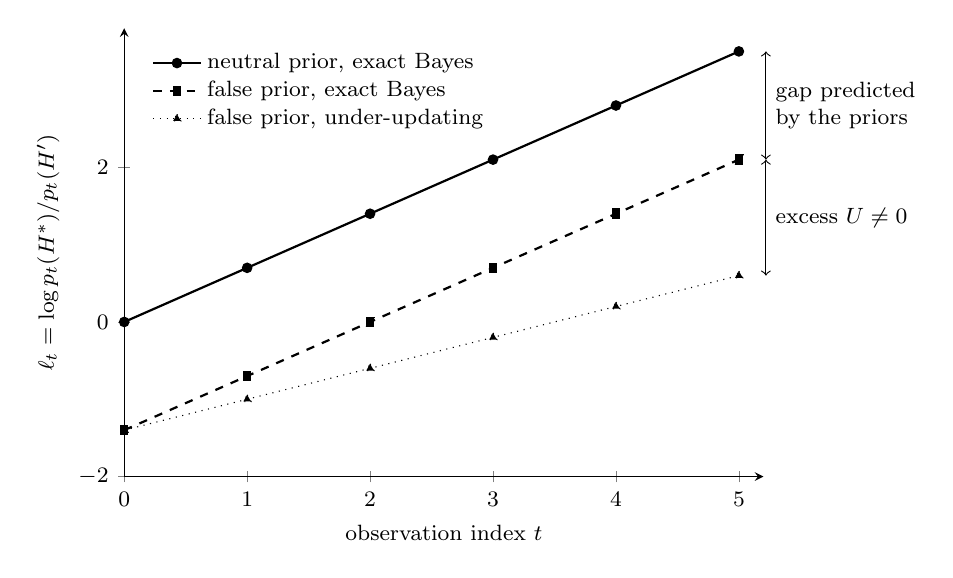
\begin{tikzpicture}
\begin{axis}[
  width=0.80\columnwidth, height=0.60\columnwidth,
  xlabel={observation index $t$},
  ylabel={$\ell_t=\log p_t(H^*)/p_t(H')$},
  xmin=0, xmax=5.2, ymin=-2, ymax=3.8,
  xtick={0,1,...,5}, ytick={-2,0,2},
  axis lines=left, axis line style={thin},
  tick label style={font=\footnotesize}, label style={font=\footnotesize},
  legend style={at={(0.03,0.97)},anchor=north west,font=\footnotesize,draw=none,fill=none,row sep=-1pt},
  legend cell align=left,
  clip=false,
]
\addplot[black, thick, mark=*, mark size=1.5pt] coordinates {(0,0) (1,0.7) (2,1.4) (3,2.1) (4,2.8) (5,3.5)};
\addlegendentry{neutral prior, exact Bayes}
\addplot[black, thick, dashed, mark=square*, mark size=1.5pt] coordinates {(0,-1.4) (1,-0.7) (2,0) (3,0.7) (4,1.4) (5,2.1)};
\addlegendentry{false prior, exact Bayes}
\addplot[black, thin, dotted, mark=triangle*, mark size=1.6pt] coordinates {(0,-1.4) (1,-1.0) (2,-0.6) (3,-0.2) (4,0.2) (5,0.6)};
\addlegendentry{false prior, under-updating}
\draw[<->,thin] (axis cs:5.22,2.1) -- (axis cs:5.22,3.5) node[midway,right,font=\footnotesize,align=left] {gap predicted\\by the priors};
\draw[<->,thin] (axis cs:5.22,0.6) -- (axis cs:5.22,2.1) node[midway,right,font=\footnotesize,align=left] {excess $U\neq 0$};
\end{axis}
\end{tikzpicture}
